\chapter{Obradba audio signala}

Nakon otvaranja audio datoteke započinje proces obradbe zvučnog signala. Audio biblioteka \textit{SoundFile} koristi se za učitavanje audio datoteke i pozivom \lstinline|sf.read(file_path)| dobivaju se matrica amplituda i frekvencija uzorkovanja. Dobivena matrica reprezentacija je audio signala u vremenskoj domeni, odnosno prikazuje glasnoću (amplitudu) zvuka dok se mijenja u vremenu. Amplituda jednaka nuli označava tišinu.

Za analizu odnosa amplitude i frekvencije signala potrebno je transformirati signal u frekvencijsku domenu za prikaz frekvencija koje se nalaze u signalu. Fourierovom transformacijom signal se dekomponira u odgovarajuće frekvencije. Biblioteka \textit{Scipy} sadrži ugrađenu funkciju za brzu Fourierovu transformaciju. 

Dobivene matrice iscrtavaju se grafički pomoću biblioteke \textit{matplotlib}. Koristeći funkciju \lstinline|matplotlib.plot()| prikazuju se tri grafa:
\begin{itemize}
	\item \textit{Audio}: prikaz samog zvučnog zapisa u vremenskoj domeni,
	\item \textit{FFT}: prikaz zvučnog zapisa u frekvencijskoj domeni dobiven Fourierovom transformacijom,
	\item \textit{Spectrogram}: prikaz spektra frekvencija signala koji se mijenja s vremenom.
\end{itemize}

Prema teoremu Nyquist-Shannon, valni oblik mora se uzorkovati frekvencijom barem dva puta većom od frekvencije signala, odnosno barem 16 kHz. Grafovi stoga prikazuju frekvencije do 8 kHz. Međutim, prikaz frekvencija na grafovima ograničen je na 2 kHz jer zvuk koji čovjek može proizvesti rijetko prelazi tu frekvenciju, stoga su frekvencije iznad 2 kHz redundantne i mogu se ukloniti. 

Na slici \ref{fig:analyse_example} prikazan je primjer zvučnog zapisa koji je učitan u aplikaciju pomoću funkcije \lstinline|filedialog.askopenfilename()| iz standardne Python biblioteke \textit{tkinter}. Na grafu zvučnog zapisa u frekvencijskoj domeni također je istaknuta frekvencija na kojoj je vrijednost funkcije maksimalna. Ovaj je podatak koristan pri određivanju dominantne frekvencije u zvučnom zapisu. 


\begin{figure}[ht]
	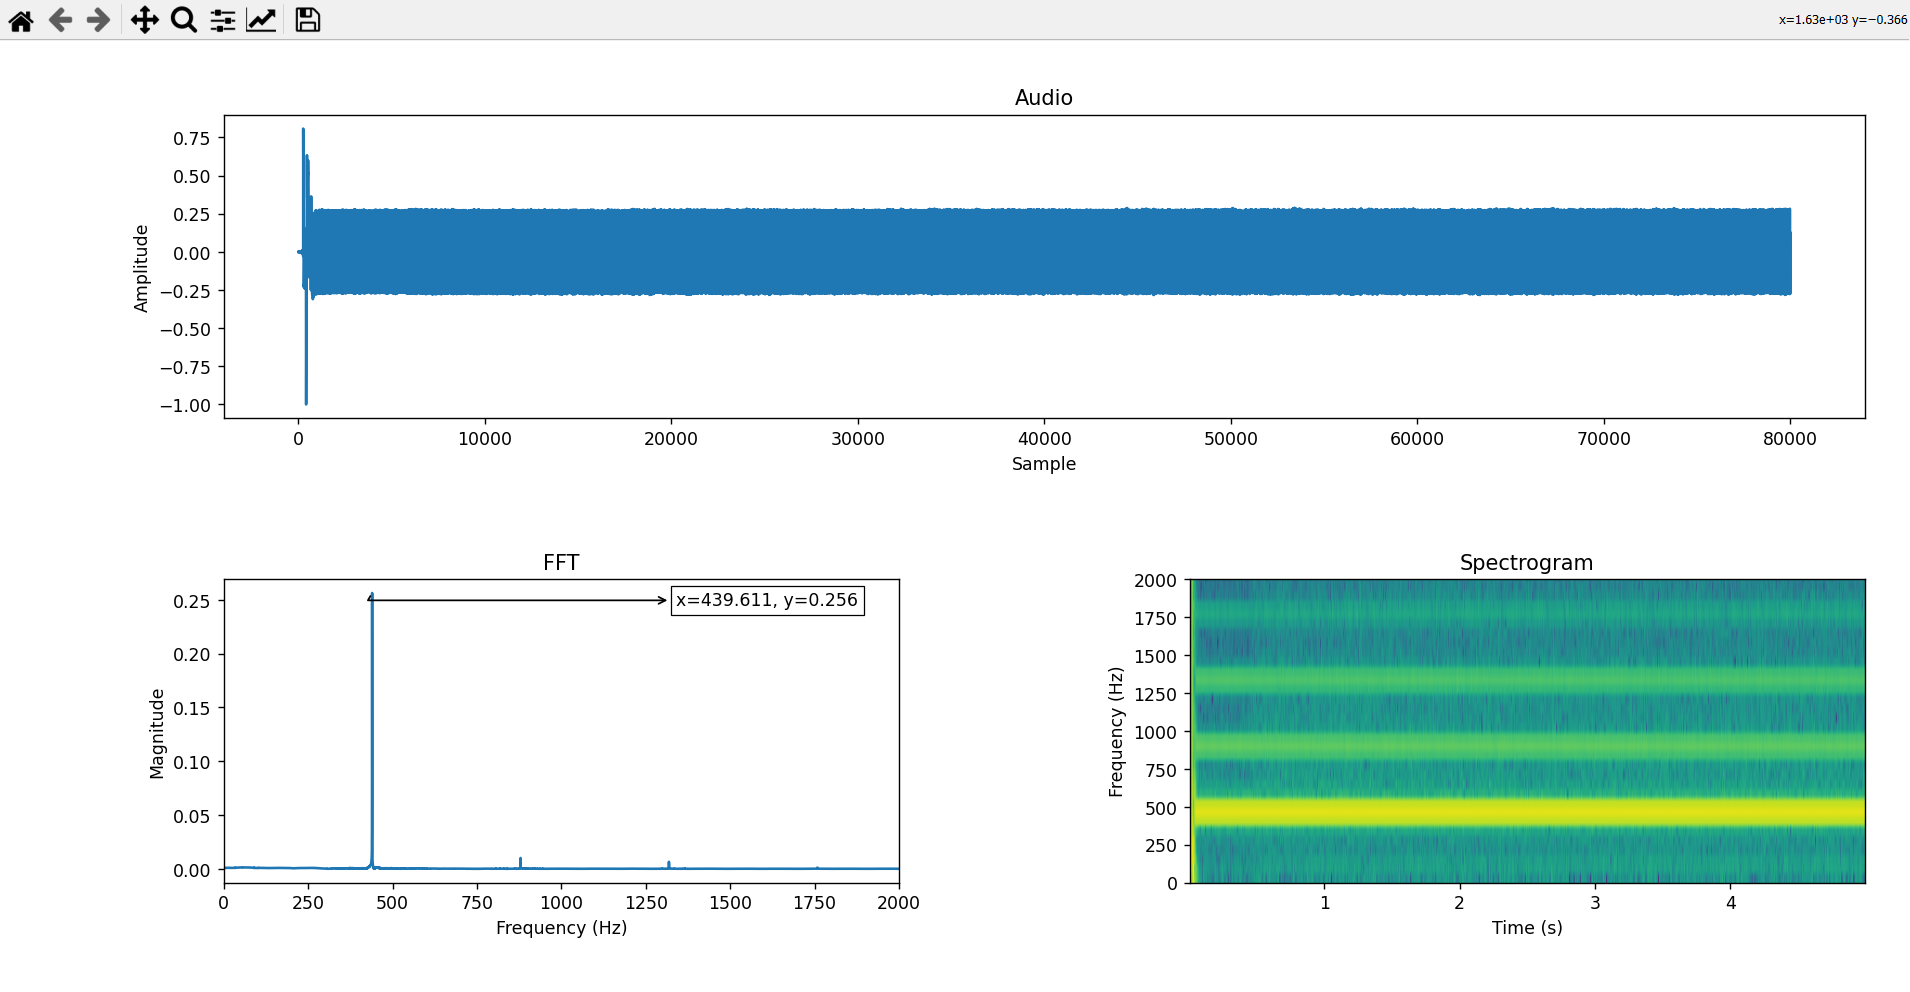
\includegraphics[width=\linewidth]{imgs/analyse_example}
	\caption{Primjer prikaza analize zvučnog zapisa}
	\label{fig:analyse_example}
\end{figure}

\section{Odnos intenziteta zvuka i udaljenosti}

Za analizu ovisnosti intenziteta zvuka o udaljenosti potrebno je pri konstantnoj frekvenciji periodično mijenjati udaljenost i mjeriti intenzitet zvuka u svakoj iteraciji. Za zvuk je odabran ton A4, odnosno zvuk s konstantnom frekvencijom od 440 Hz. Početna udaljenost izvora zvuka od mikrofona je 5 centimetara, a povećavana je za 5 centimetara u svakoj iteraciji sve do udaljenosti od 100 centimetara, odnosno 1 metra. 

Za dobivanje intenziteta svakog zvučnog zapisa korišten je \textit{Audacity}, programski paket otvorenog koda za snimanje i  uređivanje audio signala. Program nudi mogućnost analize frekvencije zvučnog zapisa i iscrtavanja grafa ovisnosti intenziteta zvuka o frekvenciji. Za dobivanje željene vrijednosti intenziteta potrebno je iz iscrtanog grafa u programu pročitati tu vrijednost pri frekvenciji od 440 Hz. Nula je postavljena za maksimalnu glasnoću, stoga su vrijednosti intenziteta zvuka prikazani u negativnoj skali. 

Provedena je analiza nad 20 zvučnih zapisa i dobivene su vrijednosti grafički prikazane u donjoj tablici. Budući da program \textit{Audacity} koristi mjerilo intenziteta zvuka u digitalnoj domeni, čiji je referentni maksimum 0 dB te minimum -100 dB, dobivene vrijednosti prikazane su negativnom skalom. 

\begin{tikzpicture}
	\begin{axis}[
		title = {Graf ovisnosti intenziteta zvuka o udaljenosti},
		xlabel=Udaljenost (cm),
		ylabel=Intenzitet zvuka (dB),
		width = 0.9\textwidth,
		height = 0.5\textwidth]
		\addplot table [y=L, x=$d$]{data.dat};
	\end{axis}
\end{tikzpicture}

Analizom grafa može se uočiti da postoji obrnuto proporcionalna ovisnost između intenziteta zvuka i udaljenosti izvora od mikrofona - što je izvor dalji od mikrofona, to je intenzitet slabiji. Dobiveni rezultati u skladu su sa zakonom inverznog kvadrata, koji tvrdi da je određena fizikalna veličina obrnuto proporcionalna kvadratu udaljenosti od izvora te fizikalne veličine: 

\begin{equation}
	intenzitet \propto \dfrac{1}{{udaljenost}^2}
\end{equation}

Uzevši u obzir referentne minimume i maksimume, dobiveni rezultati pokazuju da mikrofon dobro prima audio signal i na udaljenosti od jednog metra. Time je dokazano da je mikrofon dovoljno osjetljiv za potrebe ovog sustava.

\section{Obrada zvučnih zapisa hrkanja}

Budući da pri snimanju zvuka mikrofon snimi i neželjene frekvencije, potrebno ih je filtrirati. Za filtriranje odabrana je frekvencija od 50 Hz, što je frekvencija gradske mreže u Hrvatskoj i uzročnik najviše smetnji pri obradi zvučnog signala. Slike \ref{fig:with_notch} i \ref{fig:without_notch} prikazuju bitne razlike u očitanim frekvencijama. Na slici \ref{fig:without_notch}, koja prikazuje graf bez primjene filtra, vidljivo je da je maksimalna vrijednost na frekvenciji oko 50 Hz, što je upravo frekvencija koja je odabrana za filtriranje. Slika \ref{fig:with_notch} prikazuje graf s primjenom \textit{notch} filtra (pojasna brana), i na njoj se jasno vidi koja je stvarna frekvencija za maksimalnu vrijednost grafa. 

\begin{figure}[ht]
	\begin{minipage}[t]{0.5\textwidth}
		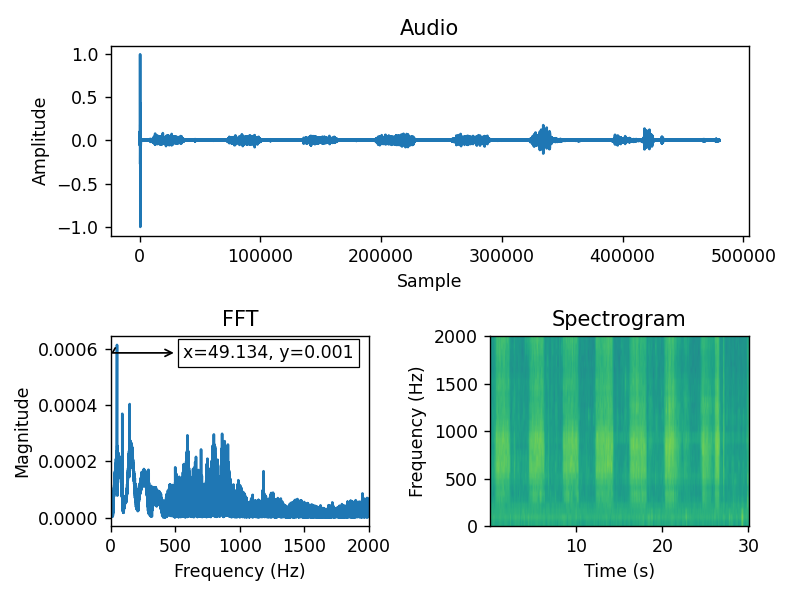
\includegraphics[width=\linewidth]{imgs/without_notch}
		\caption{Analiza bez \textit{notch} filtra}
		\label{fig:without_notch}
	\end{minipage}
	\hspace*{\fill}
	\begin{minipage}[t]{0.5\textwidth}
		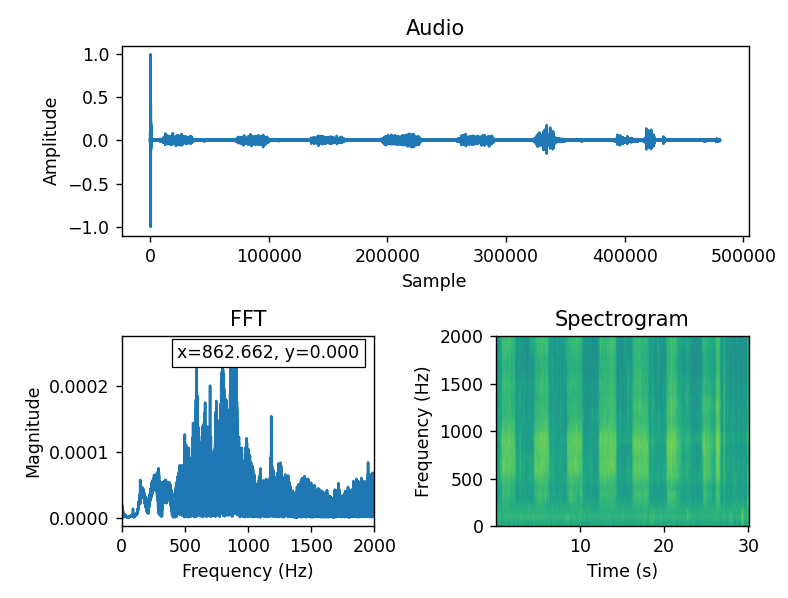
\includegraphics[width=\linewidth]{imgs/with_notch}
		\caption{Analiza s \textit{notch} filtrom}
		\label{fig:with_notch}
	\end{minipage}
\end{figure}

Pojasna brana je pojasni filtar koji kroz većinu frekvencija ostane nepromijenjen, ali prigušuje one u određenom rasponu. Suprotan je propusnom filtru koji ima cilj propuštanja željenih frekvencija. Pojasni filtri odbijaju odnosno prigušuju signale u određenom frekvencijskom pojasu koji se naziva frekvencijski raspon zaustavnog pojasa i propuštaju signale iznad i ispod tog pojasa \cite{notch}.  U nastavku je prikazana prijenosna funkcija filtra:

\begin{equation}
	H(s) = \dfrac{s^2 + \omega_0^2}{s^2 + \omega_c s + \omega_0^2}
\end{equation}

\noindent gdje je \(\omega_0\) središnja frekvencija koju se želi ukloniti, a \(\omega_c\) je širina odbijenog frekvencijskog pojasa.  Funkcija \lstinline|iirnotch()| prima središnju frekvenciju za ukloniti, faktor kvalitete i frekvenciju uzorkovanja. Funkcija vraća dva koeficijenta koje prima funkcija \lstinline|filtfilt()|. Ova funkcija primjenjuje linearni digitalni filtar na ulazni signal. Dobivenim koeficijentima koji služe kao brojnik i nazivnik prijenosne funkcije filtrira ulazni signal i vraća ga u filtriranom obliku nad kojim se dalje može pozvati funkcija za Fourierovu transformaciju \cite{scipy}. 

\begin{lstlisting}[language=Python, caption={Primjena \textit{notch} filtra i Fourierove transformacije}]
	b, a = iirnotch(50, 50/len(samples), sampling_rate)
	notch = filtfilt(b, a, samples)
	yf = fft(notch)
	xf = np.linspace(start=0.0, stop=1.0/(2.0*T), num=n//2)
\end{lstlisting}

Razvojnim sustavom STM32WB5MM-DK snimljeno je 27 zvučnih zapisa hrkanja različitih osoba. Budući da je vrlo malen uzorak, zvučni zapisi podijelit će se isključivo na palatalno i nepalatalno hrkanje. Od snimljenih zvučnih zapisa samo su 4 imala frekvenciju hrkanja 500 Hz ili niže, što znači da je nepalatalno hrkanje unutar odabranog uzorka daleko učestalije od palatalnog.

Uzme li se u obzir istraživanje vezano uz nazendoskopiju, 4 zvučna zapisa su kombinirano hrkanje nepca i jezika, dok njih 11 pripada kategoriji hrkanja u korijenu jezika. Ostali zapisi nemaju frekvencije koje su usporedive s rezultatima ovog istraživanja.